\documentclass[aspectratio=169]{beamer}
% created by Ye Tao 
% at Oct 27 2018.
% for the use of ECE551 recitation at Duke.
%
% For more themes, color themes and font themes, see:
% http://deic.uab.es/~iblanes/beamer_gallery/index_by_theme.html
%
\mode<presentation>
{
  \usetheme{Boadilla}      % or try Darmstadt, Madrid, Warsaw, ...
  \usecolortheme{default} % or try albatross, beaver, crane, ...
  \usefonttheme{default}  % or try serif, structurebold, ...
  \setbeamertemplate{navigation symbols}{}
  \setbeamertemplate{caption}[numbered]
  \setbeamercolor{footline}{fg=blue}
  \setbeamertemplate{footline}[frame number]
  \setbeamersize{text margin left=2em,text margin right=2em}
} %https://www.overleaf.com/4781826268dvwjjbjvxdvn

\usepackage[english]{babel}
\usepackage[utf8x]{inputenc}
\usepackage{comment}
% url package setting
\usepackage{hyperref}
\usepackage{listings}
%\renewcommand{\ttdefault}{blg}
\usepackage{inconsolata}
  \lstset{language=C++, basicstyle=\ttfamily}
\usepackage{graphicx}
  \graphicspath{{./figs/}}

\title[]{ECE 551 Recitation \\ Linked List \& BST}

\author{Ye Tao}
\institute{Adapted from Ian Kaszubski \& George Mappouras}
\date{\today}

\begin{document}
\begin{frame}
  \titlepage
\end{frame}

\begin{frame}{Outline}
  \tableofcontents
\end{frame}

\section{Linked List}
\subsection{Linked list overview}

\begin{frame}{Overview of Linked List}
  \begin{block}{What is a linked list?}
    \begin{itemize}
    \item<2-> A structure which is a linear sequence of nodes connected by pointers
    \item<3-> Common types: singly linked list, doubly linked list
    \item<4>  Other variation: circular link list 
    \end{itemize}
  \end{block}
  \begin{figure}[h]
    \centering
    \includegraphics<2->[scale=0.6]{linked-list}
  \end{figure}
\end{frame}

%% \begin{frame}{implement linked list class in C++}
%%     \begin{block}{Node class}
%%         \begin{itemize}
%%             \item data
%%             \item prev (for doubly linked list)
%%             \item next
%%         \end{itemize}
%%     \end{block}

%%     \begin{itemize}
%%         \item head 
%%         \item tail 
%%         \item size (track of number of nodes)
%%     \end{itemize}
%% \end{frame}

%% \begin{frame}{implement linked list class in C++}
%%   Let's first define a singly linked list:
%%   \begin{figure}
%%     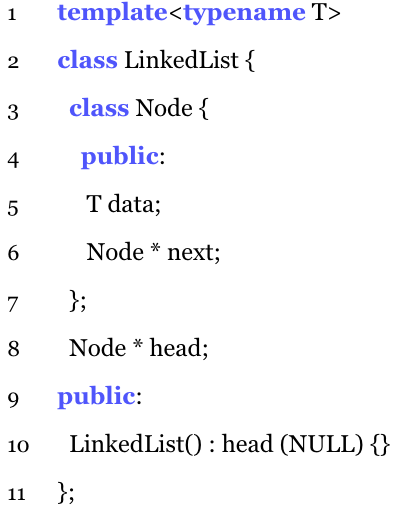
\includegraphics[height=0.8\textheight]{code_ll2.png}
%%   \end{figure}
%% \end{frame}

\begin{frame}[fragile]{Access specifiers of node class}
  \begin{columns}
  \begin{column}{0.45\textwidth}
  \begin{lstlisting}
    template<typename T>
    class LinkedList {
      //public/private?
      class Node {
        //public/private?
        T data;
        Node * next;
        Node * prev;
      };
    };
  \end{lstlisting}
  \end{column}

  \begin{column}{0.55\textwidth}
  \begin{block}{Should the Node subclass be public or private?
      \\How about its members?}
    \begin{itemize}
    \item<2-> Node class is private member of LinkedList class---cannot be accessed/changed outside of LinkedList class
    \item<3-> Fields of Node class are public---can be directly accessed/changed by LinkedList class
    \item<4-> Node class is recursively defined
    \end{itemize}
  \end{block}
  \end{column}
  \end{columns}
\end{frame}

\subsection{Linked list operations}

%% \begin{frame}{summary of common operations}
%%     \begin{enumerate}
%%         \item Add Node to the front 
%%         \item Add Node to the back
%%         \item Proper Destructor
%%         \item Add node in sorted list
%%         \item Iterators
%%         \item Reverse List
%%     \end{enumerate}
%% \end{frame}

\begin{frame}{Let's show a Linked List example}
    \begin{block}{VisuAlgo}
         visualization of data structure and algorithms: \url{https://visualgo.net/en}
    \end{block}
    \begin{block}{Visualization of Doubly Link list}
        \url{https://visualgo.net/en/list}
    \end{block}
\end{frame}

% show LL codes below
%% \begin{frame}{Add Node to the front}
%%         \begin{figure}
%%             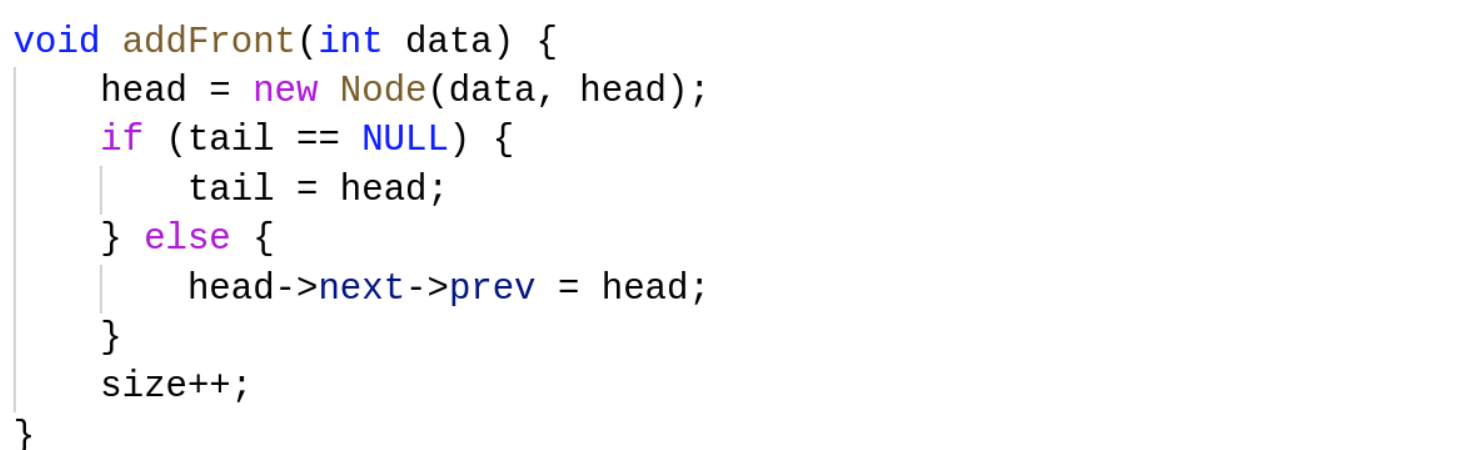
\includegraphics[width=1.5\textwidth]{LL_addfront.png}
%%     \end{figure}
%% \end{frame}

%% \begin{frame}{Add Node to the Back}
%%         \begin{figure}
%%             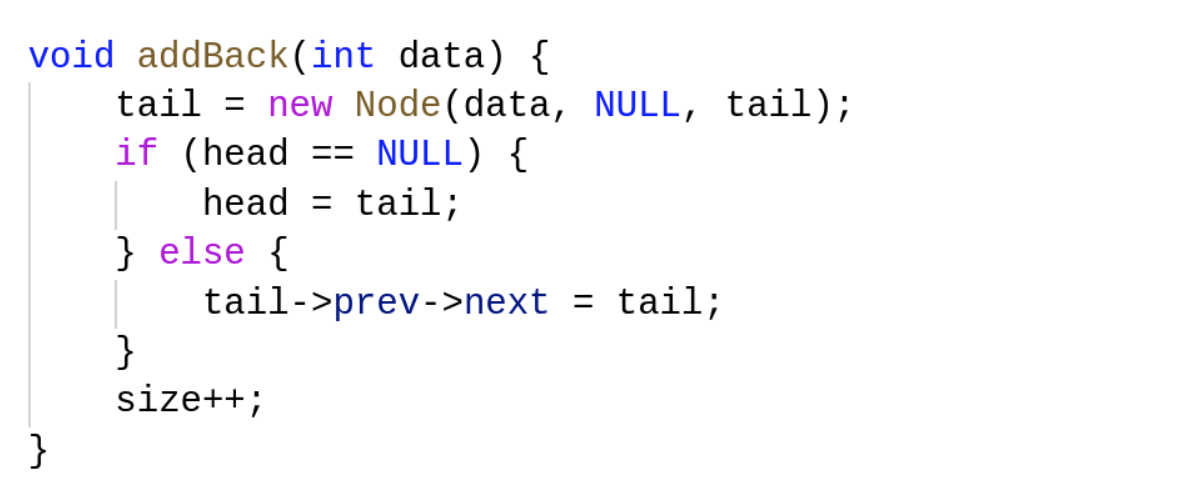
\includegraphics[width=1.3\textwidth]{LL_addback.png}
%%     \end{figure}
%% \end{frame}

%% \begin{frame}{Proper Destructor}
%%         \begin{figure}
%%             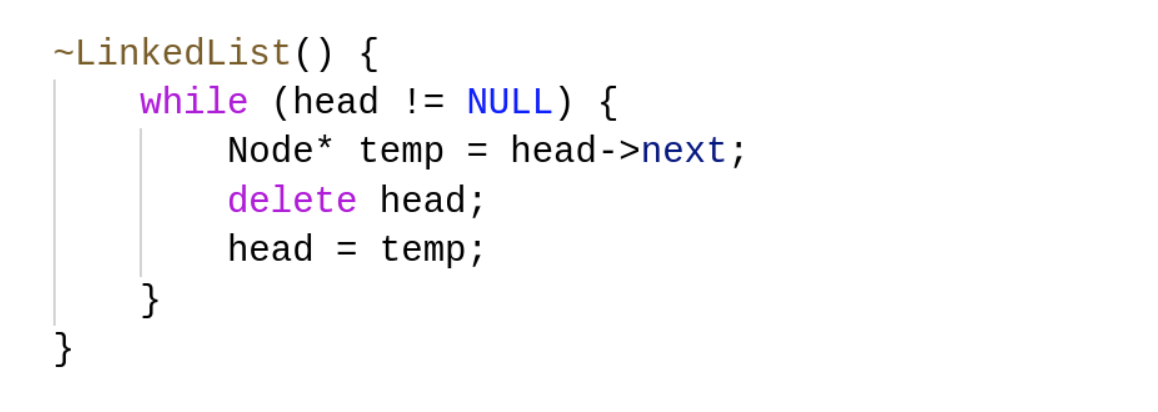
\includegraphics[width=1.3\textwidth]{LL_destructor.png}
%%     \end{figure}
%% \end{frame}

%% \begin{frame}{Add node in sorted list}
%%   \begin{figure}
%%     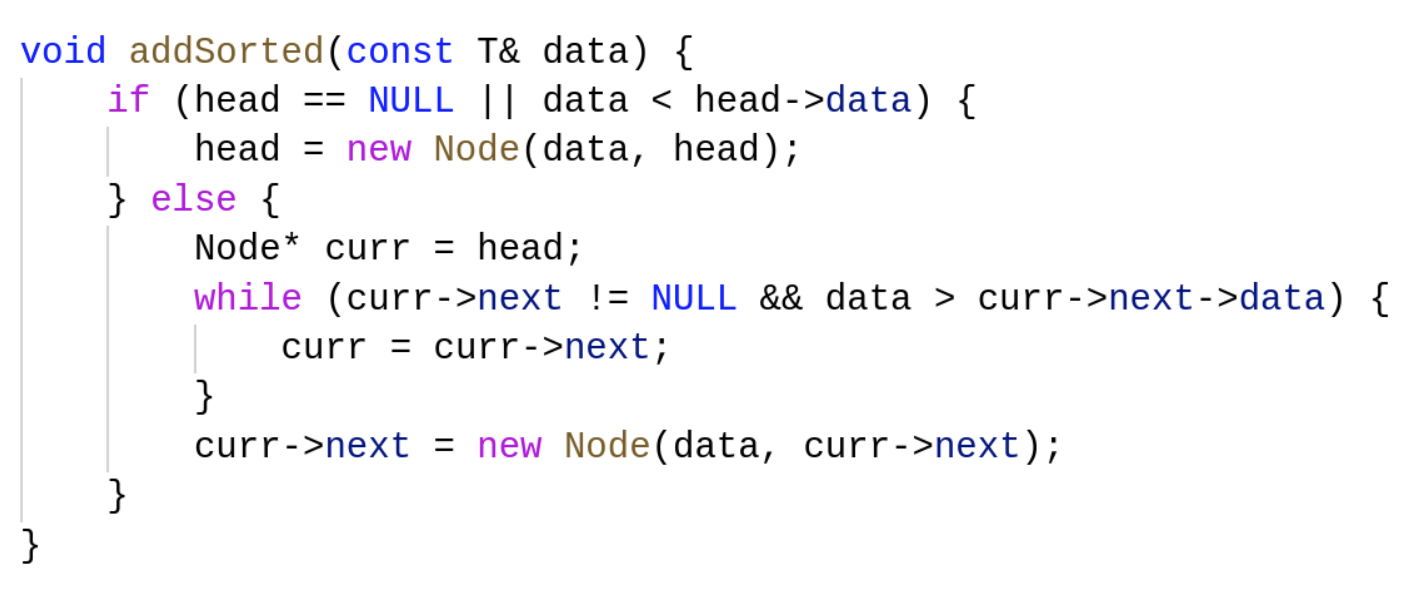
\includegraphics[width=0.9\textwidth]{LL_addsorted.png}
%%   \end{figure}
%% \end{frame}

%% \begin{frame}{Iterators}
%%   \begin{figure}
%%     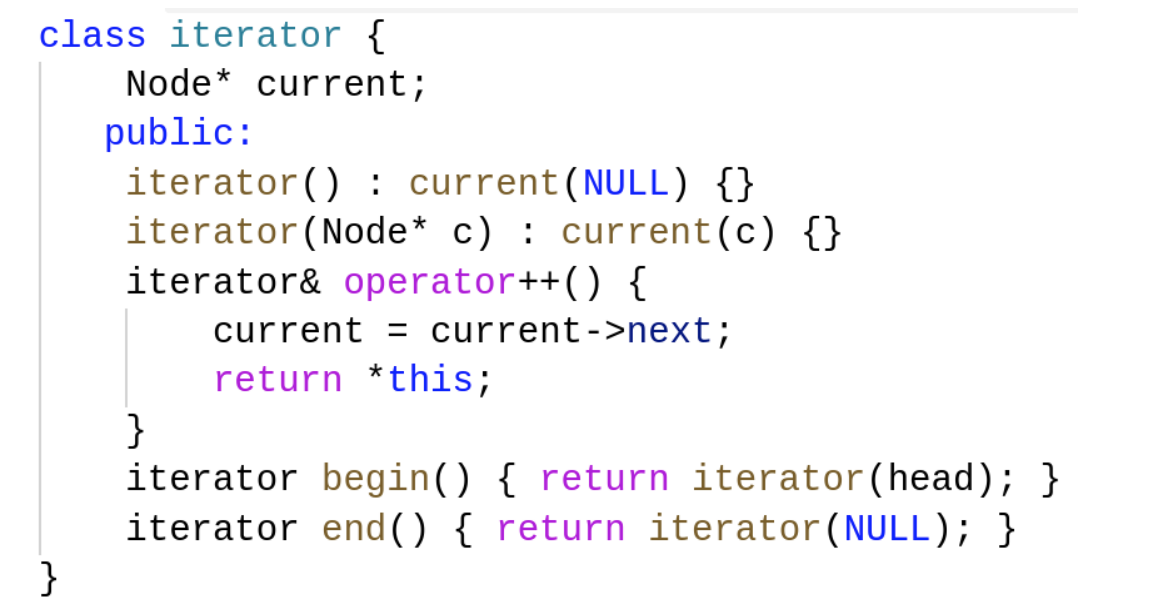
\includegraphics[width=\textwidth]{LL_iterator.png}
%%   \end{figure}
%% \end{frame}

%% \begin{frame}{Reverse Linked list}
%%   \begin{figure}
%%     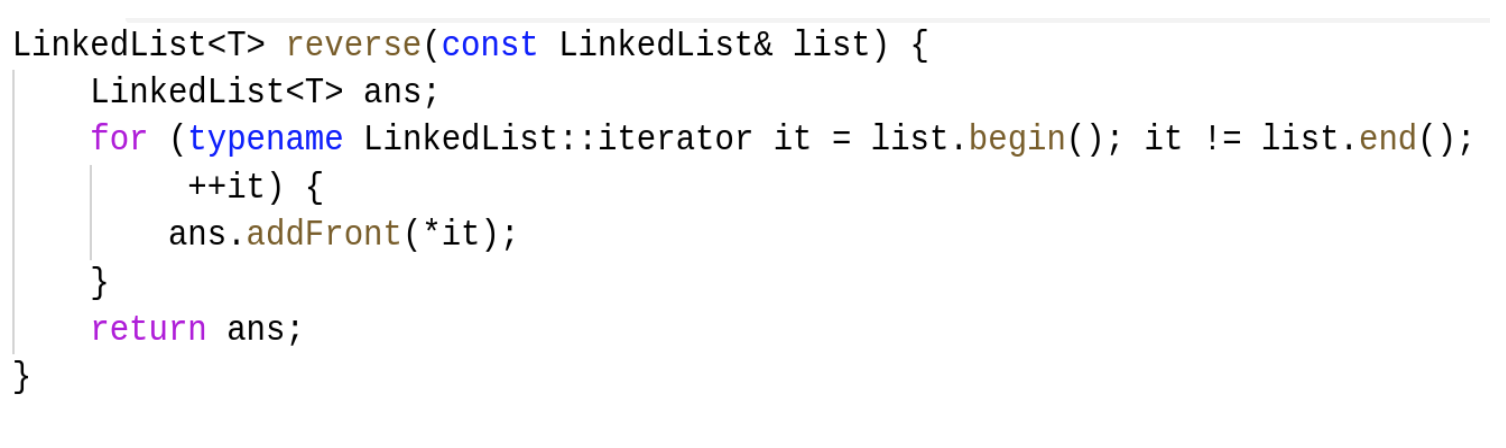
\includegraphics[width=\textwidth]{LL_reverse.png}
%%   \end{figure}
%% \end{frame}

\begin{frame}[fragile]{Linked list iterator}
Now you write one!
  \begin{lstlisting}
class iterator {
  Node * current;
public:
  iterator() : current(NULL) {}
  iterator(Node * c) : current(c) {}
  iterator & operator++();
  bool operator==(const iterator & rhs) const;
  iterator begin();
  iterator end();
};
  \end{lstlisting}
\end{frame}

\begin{frame}[fragile]{Linked list iterator}
  \begin{lstlisting}
iterator & operator++() {
  current = current->next;
  return *this;
}
bool operator==(const iterator & rhs) const {
  return current == rhs.current;
}
iterator begin() {
  return iterator(head);
}
iterator end() {
  return iterator(NULL);
}
  \end{lstlisting}      
\end{frame}

\subsection{STL list}
\begin{frame}[fragile]{STL list}
  \begin{enumerate}
  \item \url{http://www.cplusplus.com/reference/list/list/}
  \item Doubly linked list
  \item \begin{verbatim}template <class T> class list;\end{verbatim}
  \end{enumerate}
\end{frame}

\section{Binary Search Tree}
\subsection{BST overview}

\begin{frame}{BST overview}
  \begin{block}{What is a binary search tree?}
    \begin{itemize}
    \item<2->Data structure designed to split search in half at each step 
    \item<3->Usually results in $\mathcal{O}(\log{N})$ time
    \item<4> Contrast with typical $\mathcal{O}(N)$ for linked list
    \end{itemize}
  \end{block}
  \begin{figure}[h]
    \centering
    \includegraphics<2->[scale=0.5]{bst}
  \end{figure}
\end{frame}

%% \begin{frame}{BST diagram}
%%         \begin{figure}
%%             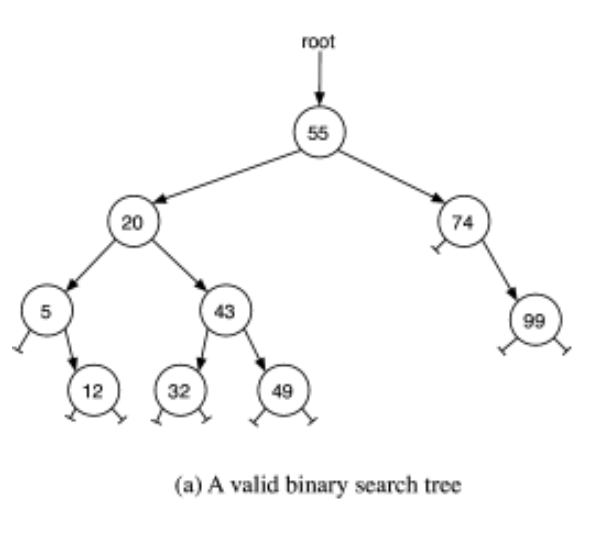
\includegraphics[width=0.6\textwidth]{BST_fig.png}
%%             \caption{From Aop}
%%     \end{figure}
%% \end{frame}

%% \begin{frame}{BST class in c++}
%%     We need:
%%     \begin{itemize}
%%         \item node class similar to Linked list.
%%             \begin{itemize}
%%                 \item left and right pointers (edges). 
%%                 \item data
%%             \end{itemize}
%%         \item root (a pointer pointing at the very top node).
%%     \end{itemize}
%% \end{frame}

%% \begin{frame}{BST class in C++}
%%         \begin{figure}
%%             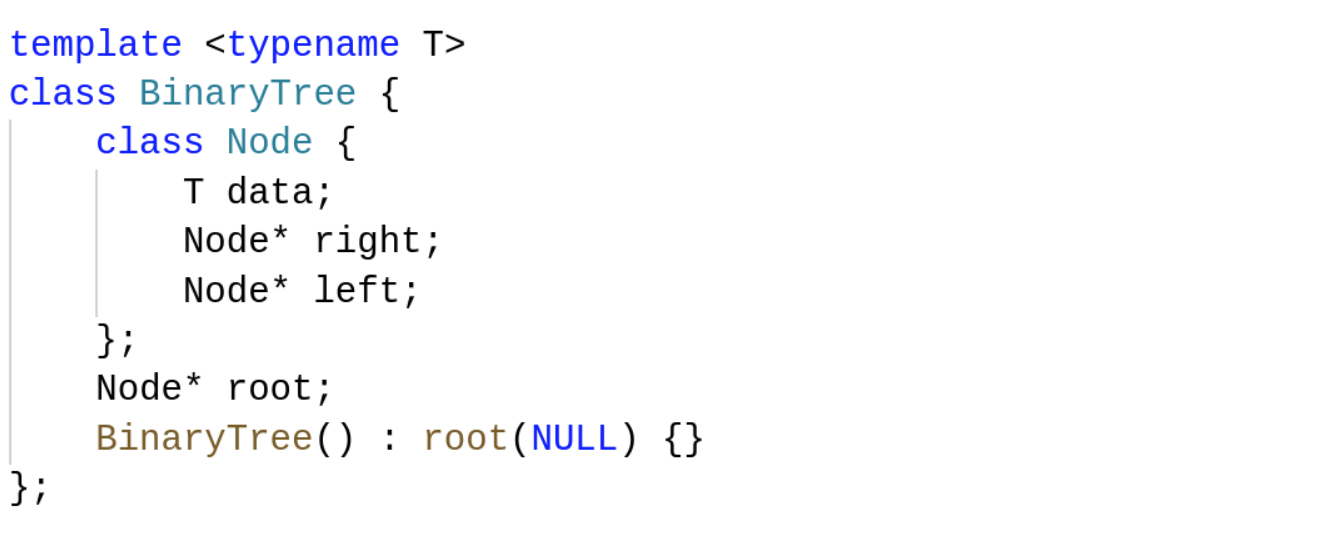
\includegraphics[width=\textwidth]{BST_class.png}
%%     \end{figure}
%% \end{frame}

%% \subsection{BST operations}
%% \begin{frame}{common operations of BST}
%%     \begin{itemize}
%%         \item Search for a node
%%         \item Adding a node 
%%         \item Removing a Node
%%     \end{itemize}
%% \end{frame}

\begin{frame}{Let's show a BST example}
    \begin{block}{VisuAlgo}
         An visualization of data structure and algorithms: \url{https://visualgo.net/en}
    \end{block}
    \begin{block}{Visualization of BST}
        \url{https://visualgo.net/en/bst?slide=1}
    \end{block}
\end{frame}

%% \begin{frame}{Search for a node}
%%         \begin{figure}
%%             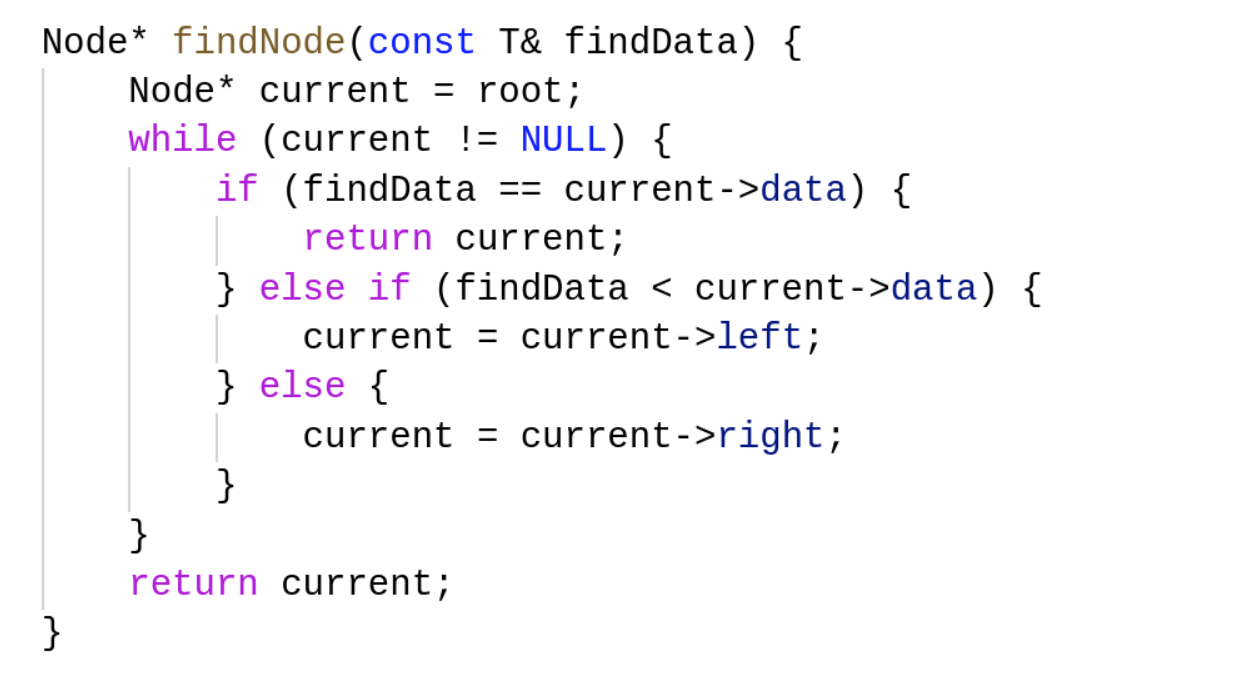
\includegraphics[width=\textwidth]{BST_find.png}
%%     \end{figure}
%% \end{frame}

%% \begin{frame}{Adding a node}
%%         \begin{figure}
%%             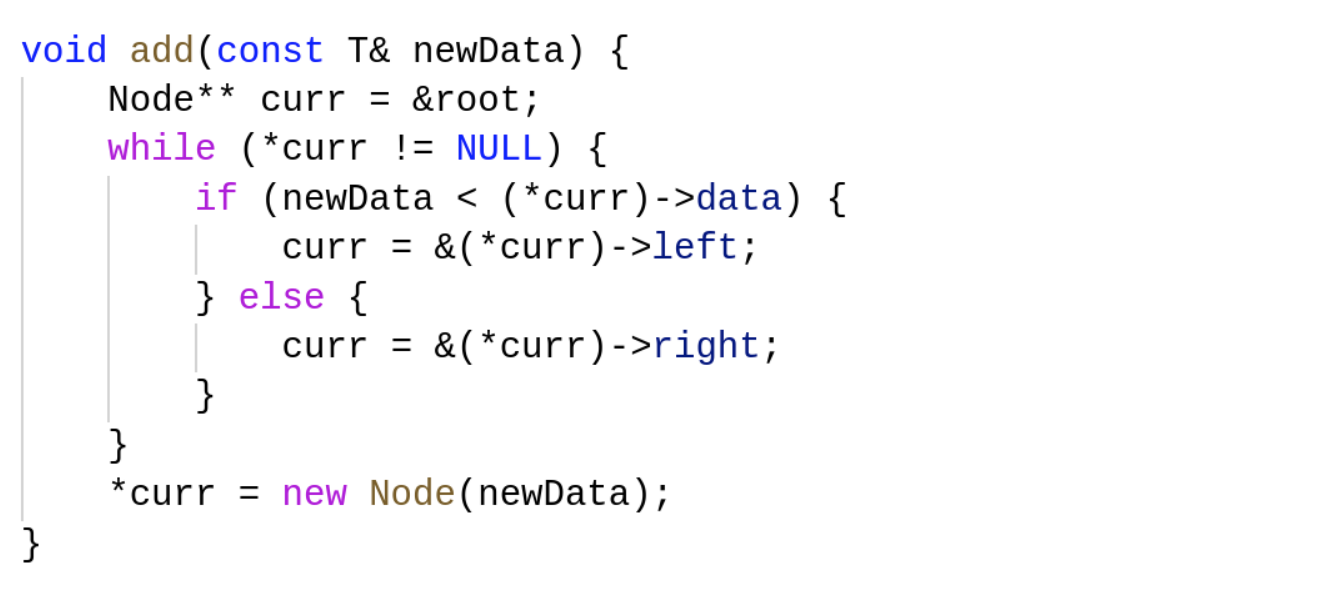
\includegraphics[width=\textwidth]{BST_add.png}
%%     \end{figure}
%% \end{frame}

%% \begin{frame}{Removing a Node}
%%     \begin{itemize}
%%         \item Removing a Node: Complex but many ways to do it but only one shown in this slide due to time limit.
%%         \item two helper functions:
%%             \begin{enumerate}
%%                 \item Find right most node. 
%%                     \begin{itemize}
%%                         \item why we need this?
%%                         \item think about how remove is performed.
%%                         % show visualization of removing nodes.
%%                     \end{itemize}
%%                 \item delete helper actually perform removing.
%%                 \item delete function calling delete helper.
%%             \end{enumerate}
%%     \end{itemize}
%% \end{frame}

%% \begin{frame}{Recursively removing a Node:  Find right most node}
%%         \begin{figure}
%%             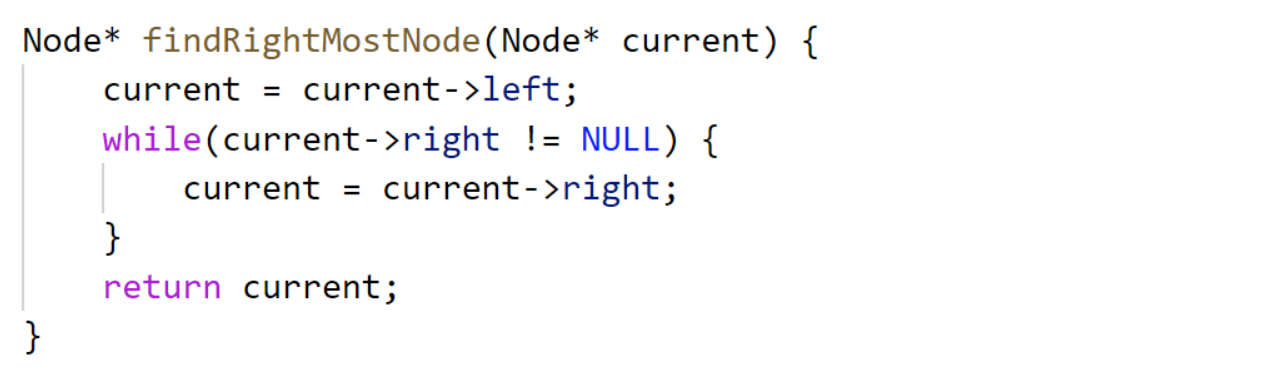
\includegraphics[width=\textwidth]{BST_FRM.png}
%%     \end{figure}
%% \end{frame}

%% \begin{frame}{Recursively removing a Node:  Find right most node}
%%         \begin{figure}
%%             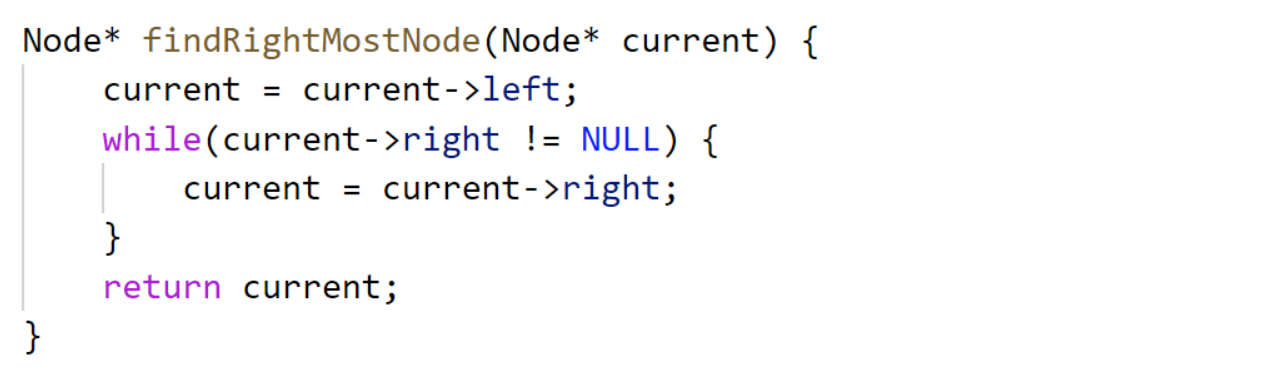
\includegraphics[width=\textwidth]{BST_FRM.png}
%%     \end{figure}
%% \end{frame}

%% \begin{frame}{Removing a Node: remove}
%%         \begin{figure}
%%             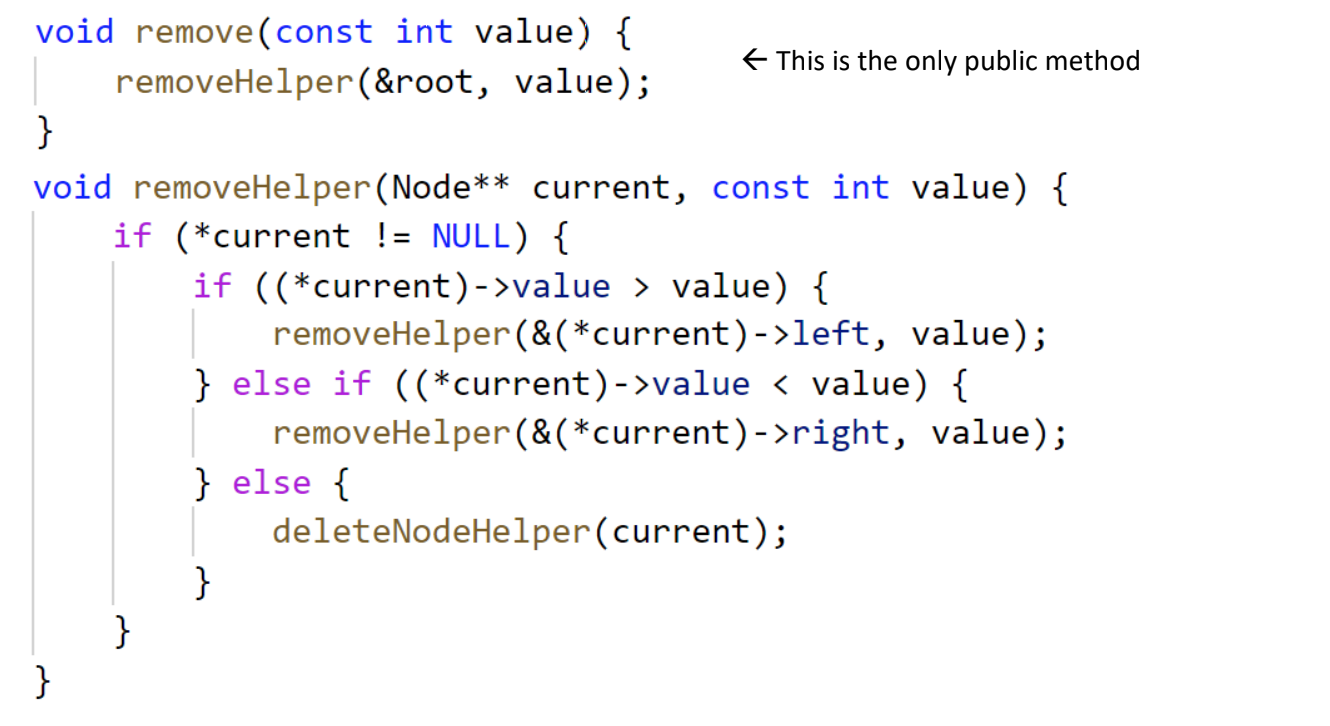
\includegraphics[width=\textwidth]{BST_remove.png}
%%     \end{figure}
%% \end{frame}

% if there are time left
\subsection{Tree traversal}
\begin{frame}{Three orders of tree traversal}
        \begin{figure}
            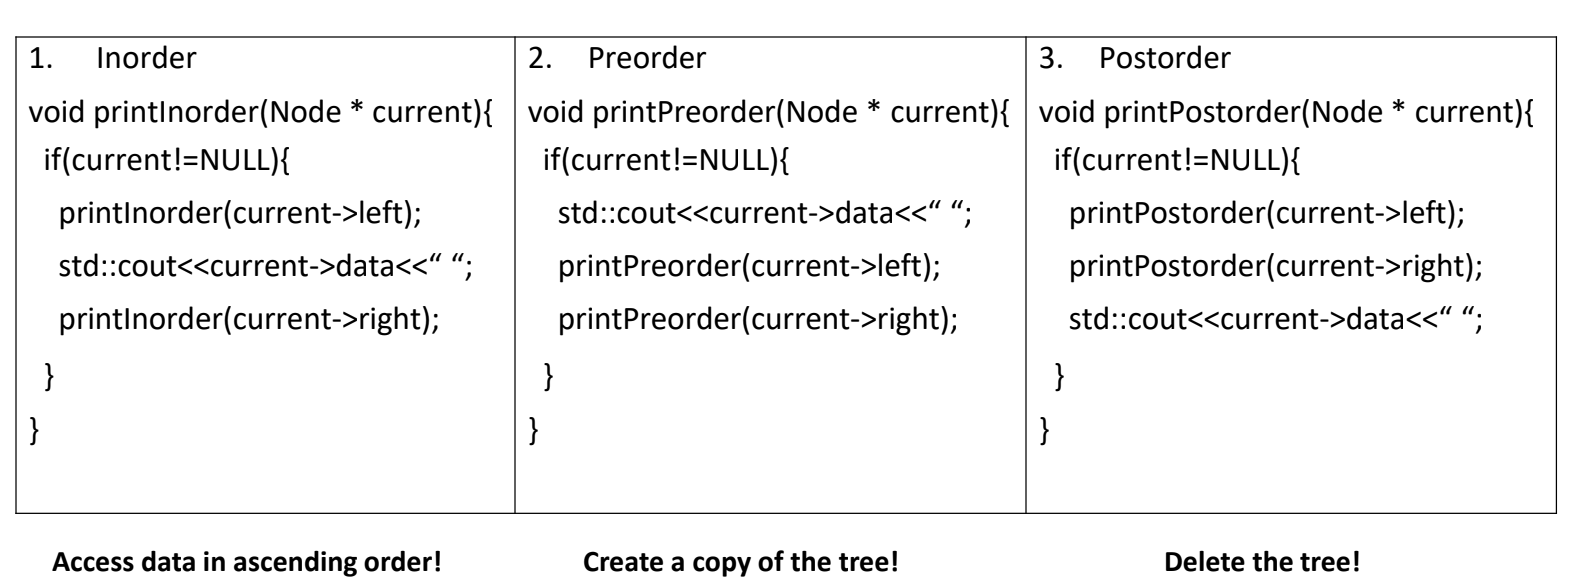
\includegraphics[width=\textwidth]{BST_traverse.png}
    \end{figure}
\end{frame}

\begin{frame}{Three orders of tree traversal}
        \begin{figure}
            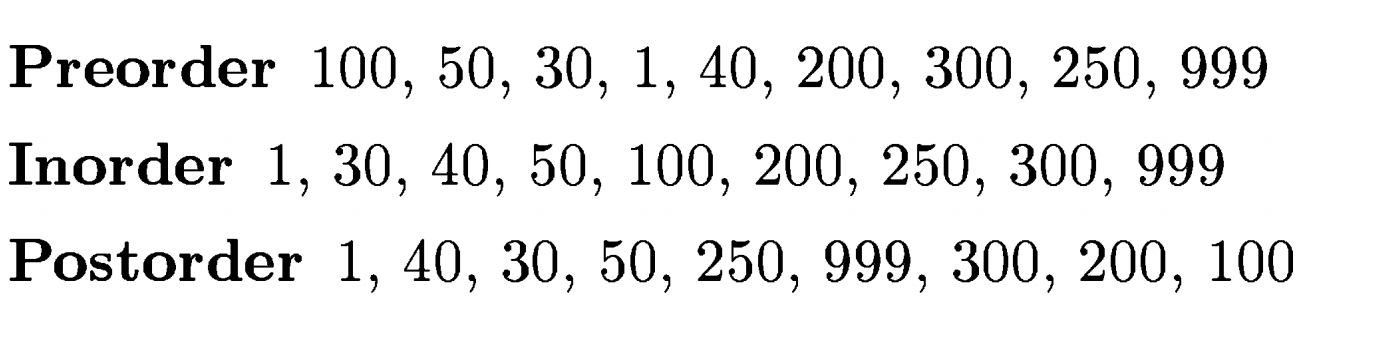
\includegraphics[width=\textwidth]{BST_order.png}
    \end{figure}
\end{frame}

\begin{frame}{STL Binary search tree?}

\begin{itemize}
    \item No such thing in C++ STL.
    \item Alternates: What you need is to find  data by a key.
        \begin{itemize}
            \item std::map, std::set, etc.
            \item they're actually implemented in red-black tree which is a variants of BST.
            \item you'll learn that in Aop chapter 27.
        \end{itemize}
\end{itemize}
    
\end{frame}

\end{document}
